













%%%%%%%%%%%%%%
% !TeX spellcheck = da_DK
%implementing document formatting:
\documentclass[a4paper,11pt,fleqn,dvipsnames,oneside,openright,oldfontcommands]{memoir} 	% Openright aabner kapitler paa hoejresider (openany begge)

\usepackage{xfrac}
\usepackage{booktabs}
\usepackage[table,xcdraw]{xcolor}

%%%%%%%%% Indsat random
%makes it possible to refer to the name of a chapter rather than just the number.
\usepackage{nameref}
\usepackage{pdfpages}
\usepackage{marvosym}
\usepackage{setspace}
\usepackage{graphicx} % For at sætte 2 billeder ved siden af hinanden

%package for writing program code in latex
\usepackage{listings}
%%%%%%%%%%%%%%%%%%%%%%

% ¤¤ Oversaettelse og tegnsaetning ¤¤ %
\usepackage[T1]{fontenc}					% Output-indkodning af tegnsaet (T1)
\usepackage[danish]{babel}					% Dokumentets sprog
\usepackage[utf8]{inputenc}					% Input-indkodning af tegnsaet (UTF8)
\usepackage{ragged2e,anyfontsize}			% Justering af elementer
\usepackage{fixltx2e}						% Retter forskellige fejl i LaTeX-kernen			
\usepackage{gensymb}						% Nu kan der skrices procent tegn med \degree				
				
																							
% ¤¤ Figurer og tabeller (floats) ¤¤ %
\usepackage{graphicx} 						% Haandtering af eksterne billeder (JPG, PNG, EPS, PDF)
%\usepackage{eso-pic}						% Tilfoej billedekommandoer paa hver side
\usepackage{wrapfig}						% Indsaettelse af figurer omsvoebt af tekst. \begin{wrapfigure}{Placering}{Stoerrelse}
\usepackage{multirow}                		% Fletning af raekker og kolonner (\multicolumn og \multirow)
\usepackage{multicol}         	        	% Muliggoer output i spalter
\usepackage{rotating}						% Rotation af tekst med \begin{sideways}...\end{sideways}
\usepackage{colortbl} 						% Farver i tabeller (fx \columncolor og \rowcolor)
\usepackage{xcolor}							% Definer farver med \definecolor. Se mere: http://en.wikibooks.org/wiki/LaTeX/Colors
\usepackage{flafter}						% Soerger for at floats ikke optraeder i teksten foer deres reference
\let\newfloat\relax 						% Justering mellem float-pakken og memoir
\usepackage{float}							% Muliggoer eksakt placering af floats, f.eks. \begin{figure}[H]
\usepackage{array,booktabs,xcolor,longtable} % kan lave \hdashline i tabellertabe
\usepackage{arydshln}
\usepackage{tabu}
\usepackage{epstopdf} 						% Muligoer brugen af eps filer i latex

	
	
% ¤¤ Matematik mm. ¤¤
\usepackage{amsmath , amsthm , amsfonts , amssymb, float, stmaryrd} 		% Avancerede matematik-udvidelser
%\usepackage{mathtools}						% Andre matematik- og tegnudvidelser
\usepackage{textcomp}                 		% Symbol-udvidelser (f.eks. promille-tegn med \textperthousand )
\usepackage{rsphrase}						% Kemi-pakke til RS-saetninger, f.eks. \rsphrase{R1}
\usepackage[version=3]{mhchem} 				% Kemi-pakke til flot og let notation af formler, f.eks. \ce{Fe2O3}
\usepackage{siunitx}						% Flot og konsistent praesentation af tal og enheder med \si{enhed} og \SI{tal}{enhed}
\sisetup{output-decimal-marker = {,}}		% Opsaetning af \SI (DE for komma som decimalseparator) 

% ¤¤ Referencer og kilder ¤¤ %
\usepackage[danish]{varioref}				% Muliggoer bl.a. krydshenvisninger med sidetal (\vref)
\usepackage[numbers]{natbib}				% Udvidelse med naturvidenskabelige citationsmodeller
%%\usepackage[sort&compress,square,comma,numbers]{natbib}
\newcommand{\citer}[1]{\citeauthor{#1},~\citeyear{#1}~\cite{#1}}

%\DeclareRobustCommand{\citer}[1]{\citeauthor{#1},~\citeyear{#1}~\cite{#1}}
											% citere i teksten: "Et studie af 'forfatter', 'år' [kilde#] viser..."
%\usepackage{xr}							% Referencer til eksternt dokument med \externaldocument{<NAVN>}
%\usepackage{glossaries}					% Terminologi- eller symbolliste (se mere i Daleifs Latex-bog)
\usepackage{lastpage}					% Gør det mulig at refere til sidste side 

% ¤¤ Misc. ¤¤ %
\usepackage{listings}						% Placer kildekode i dokumentet med \begin{lstlisting}...\end{lstlisting}
\usepackage{lipsum}							% Dummy text \lipsum[..]
\usepackage[shortlabels]{enumitem}			% Muliggoer enkelt konfiguration af lister
\usepackage{pdfpages}						% Goer det muligt at inkludere pdf-dokumenter med kommandoen \includepdf[pages={x-y}]{fil.pdf}	
\pdfoptionpdfminorversion=6					% Muliggoer inkludering af pdf dokumenter, af version 1.6 og hoejere
\pretolerance=2500 							% Justering af afstand mellem ord (hoejt tal, mindre orddeling og mere luft mellem ord)


% Kommentarer og rettelser med \fxnote. Med 'final' i stedet for 'draft' udloeser hver note en error i den faerdige rapport.
\usepackage[footnote,final,danish,silent,nomargin]{fixme}		


%%%% CUSTOM SETTINGS %%%%

% ¤¤ Marginer ¤¤ %
\setlrmarginsandblock{3.0cm}{2.5cm}{*}		% \setlrmarginsandblock{Indbinding}{Kant}{Ratio}
\setulmarginsandblock{2.5cm}{3.0cm}{*}		% \setulmarginsandblock{Top}{Bund}{Ratio}
\checkandfixthelayout 						% Oversaetter vaerdier til brug for andre pakker

%	¤¤ Afsnitsformatering ¤¤ %
\setlength{\parindent}{0mm}           		% Stoerrelse af indryk
\setlength{\parskip}{3mm}          			% Afstand mellem afsnit ved brug af double Enter
\linespread{1,1}							% Linie afstand



% ¤¤ Indholdsfortegnelse ¤¤ %
\setsecnumdepth{subsection}		 			% Dybden af nummerede overkrifter (part/chapter/section/subsection)
\maxsecnumdepth{subsection}					% Dokumentklassens graense for nummereringsdybde
\settocdepth{section} 					% Dybden af indholdsfortegnelsen

% ¤¤ Lister ¤¤ %
\setlist{
  topsep=0pt,								% Vertikal afstand mellem tekst og listen
  itemsep=-1ex,								% Vertikal afstand mellem items
} 

%hyperlinks in the tabel of contents - comment this out before the report is printed.
\usepackage{hyperref}
\hypersetup{
	bookmarks = true,  % Show 'bookmark'-frame in pdf.
	colorlinks = true, % True = colored links, False = framed links.
	citecolor = black,  % Link color for references.
	linkcolor = black,  % Link color in table of contents.
	urlcolor = black,   % Link color for extern URLs.
}

% ¤¤ Opsaetning af figur- og tabeltekst ¤¤ %
\usepackage{caption}
\usepackage{subcaption}
\captionnamefont{\small\bfseries\itshape}	% Opsaetning af tekstdelen ('Figur' eller 'Tabel')
\captiontitlefont{\small}					% Opsaetning af nummerering
\captiondelim{. }							% Seperator mellem nummerering og figurtekst
\hangcaption								% Venstrejusterer flere-liniers figurtekst under hinanden
%\captionwidth{0.9\textwidth}					% Bredden af figurteksten
\setlength{\belowcaptionskip}{0pt}			% Afstand under figurteksten
\captionsetup[figure]{labelfont={bf,it},font={it}} % sætter nummer til fed og kursis. Resten til fed + skriften er mindre end resten
\captionsetup[table]{labelfont={bf,it},font={it}} 


% ¤¤ Opsaetning af listings ¤¤ %

\definecolor{commentGreen}{RGB}{34,139,24}
\definecolor{stringPurple}{RGB}{208,76,239}

\lstset{language=Matlab,					% Sprog
	basicstyle=\ttfamily\scriptsize,		% Opsaetning af teksten
	keywords={for,if,while,else,elseif,		% Noegleord at fremhaeve
			  end,break,return,case,
			  switch,function},
	keywordstyle=\color{blue},				% Opsaetning af noegleord
	commentstyle=\color{commentGreen},		% Opsaetning af kommentarer
	stringstyle=\color{stringPurple},		% Opsaetning af strenge
	showstringspaces=false,					% Mellemrum i strenge enten vist eller blanke
	numbers=left, numberstyle=\tiny,		% Linjenumre
	extendedchars=true, 					% Tillader specielle karakterer
	columns=flexible,						% Kolonnejustering
	breaklines, breakatwhitespace=true,		% Bryd lange linjer
}

% ¤¤ Navngivning ¤¤ %
\addto\captionsdanish{
	\renewcommand\appendixname{Appendiks}
	\renewcommand\contentsname{Indholdsfortegnelse}	
	\renewcommand\appendixpagename{Appendiks}
	\renewcommand\appendixtocname{Appendiks}
	\renewcommand\cftchaptername{\chaptername~}				% Skriver "Kapitel" foran kapitlerne i indholdsfortegnelsen
	\renewcommand\cftappendixname{\appendixname~}			% Skriver "Appendiks" foran appendiks i indholdsfortegnelsen
}

% ¤¤ Kapiteludssende ¤¤ %
\definecolor{numbercolor}{gray}{0.7}		% Definerer en farve til brug til kapiteludseende
\newif\ifchapternonum

\makechapterstyle{jenor}{					% Definerer kapiteludseende frem til ...
	\renewcommand\beforechapskip{0pt}
	\renewcommand\printchaptername{}
	\renewcommand\printchapternum{}
	\renewcommand\printchapternonum{\chapternonumtrue}
	\renewcommand\chaptitlefont{\fontfamily{pbk}\fontseries{db}\fontshape{n}\fontsize{20}{35}\selectfont\raggedright}
	\renewcommand\chapnumfont{\fontfamily{pbk}\fontseries{m}\fontshape{n}\fontsize{0.35in}{0in}\selectfont\color{black}}
	\renewcommand\printchaptertitle[1]{%
		\noindent
		\ifchapternonum
		\begin{tabularx}{\textwidth}{X}
			{\let\\\newline\chaptitlefont ##1\par} 
		\end{tabularx}
		\par\vskip-2.5mm\hrule
		\else
		\begin{tabularx}{\textwidth}{Xl}
			{\parbox[b]{\linewidth}{\chaptitlefont ##1}} & \raisebox{-5pt}{\chapnumfont \thechapter}
		\end{tabularx}
		\par\vskip2mm\hrule
		\fi
	}
}											% ... her

\chapterstyle{jenor}						% Valg af kapiteludseende - Google 'memoir chapter styles' for alternativer

% ¤¤ Sidehoved ¤¤ %

\makepagestyle{AAU}							% Definerer sidehoved og sidefod udseende frem til ...
\makepsmarks{AAU}{%
	\createmark{chapter}{left}{shownumber}{}{. \ }
	\createmark{section}{right}{shownumber}{}{. \ }
	\createplainmark{toc}{both}{\contentsname}
	\createplainmark{lof}{both}{\listfigurename}
	\createplainmark{lot}{both}{\listtablename}
	\createplainmark{bib}{both}{\bibname}
	\createplainmark{index}{both}{\indexname}
	\createplainmark{glossary}{both}{\glossaryname}
}
\nouppercaseheads											% Ingen Caps oenskes

\makeevenhead{AAU}{Gruppe 5406}{}{\leftmark}				% Definerer lige siders sidehoved (\makeevenhead{Navn}{Venstre}{Center}{Hoejre})
\makeoddhead{AAU}{\rightmark}{}{Aalborg Universitet}		% Definerer ulige siders sidehoved (\makeoddhead{Navn}{Venstre}{Center}{Hoejre})
\makeevenfoot{AAU}{\thepage}{}{}							% Definerer lige siders sidefod (\makeevenfoot{Navn}{Venstre}{Center}{Hoejre})
\makeoddfoot{AAU}{}{}{\thepage}								% Definerer ulige siders sidefod (\makeoddfoot{Navn}{Venstre}{Center}{Hoejre})
\makeheadrule{AAU}{\textwidth}{0.5pt}						% Tilfoejer en streg under sidehovedets indhold
\makefootrule{AAU}{\textwidth}{0.5pt}{1mm}					% Tilfoejer en streg under sidefodens indhold

\copypagestyle{AAUchap}{AAU}								% Sidehoved for kapitelsider defineres som standardsider, men med blank sidehoved
\makeoddhead{AAUchap}{}{}{}
\makeevenhead{AAUchap}{}{}{}
\makeheadrule{AAUchap}{\textwidth}{0pt}
\aliaspagestyle{chapter}{AAUchap}							% Den ny style vaelges til at gaelde for chapters
% ... her

\pagestyle{AAU}												% Valg af sidehoved og sidefod


%%%% CUSTOM COMMANDS %%%%

% ¤¤ Billede hack ¤¤ %
\newcommand{\figur}[4]{
		\begin{figure}[H] \centering
			\includegraphics[width=#1\textwidth]{billeder/#2}
			\caption{#3}\label{#4}
		\end{figure} 
}

% ¤¤ Specielle tegn ¤¤ %
\newcommand{\decC}{^{\circ}\text{C}}
\newcommand{\dec}{^{\circ}}
\newcommand{\m}{\cdot}


%%%% ORDDELING %%%%

\hyphenation{}

%%%%Fra engelsk til dansk i \autoref{•} %%%%
\renewcommand{\figureautorefname}{Figur}
\renewcommand{\sectionautorefname}{Afsnit}
\renewcommand{\subsectionautorefname}{Afsnit}
\renewcommand{\subsubsectionautorefname}{Afsnit}
\renewcommand{\tableautorefname}{Tabel}
\renewcommand{\appendixautorefname}{Appendiks}
\renewcommand{\equationautorefname}{Ligning}
\renewcommand{\itemautorefname}{Punkt}
\renewcommand{\chapterautorefname}{Kapitel}
\raggedbottom
%Figure references:
\newcommand{\figref}[1]{figur~\ref{#1}}

%Figure references after full stop/period:
\newcommand{\Figref}[1]{Figur~\ref{#1}}

%Table references:
\newcommand{\tabref}[1]{tabel~\ref{#1}}

%Table references after full stop/period:
\newcommand{\Tabref}[1]{Tabel~\ref{#1}}

%Appendix references:
\newcommand{\appref}[1]{appendiks~\ref{#1}}

%Appendix references after full stop/period:
\newcommand{\Appref}[1]{Appendiks~\ref{#1}}

%Section references:
\newcommand{\secref}[1]{afsnit~\ref{#1}}

%Section references:
\newcommand{\Secref}[1]{Afsnit~\ref{#1}}

%chapter references: 
\newcommand{\chapref}[1]{kapitel~\ref{#1}}

%chapter references: 
\newcommand{\Chapref}[1]{Kapitel~\ref{#1}}


%Units:
%inserting '\omit' before '{\put' prior ot final compile will fix allignment (and generate errors)
\newcommand{\unit}[1]{{\put(300,0){$\hfill\left[\: #1 \:\right]$}}}

%Text:
\newcommand{\tx}[1]{\text{#1}}

%Equation references:
%1 equation:
\renewcommand{\eqref}[1]{ligning~(\ref{#1})}
%2 equations:
\newcommand{\eqrefTwo}[2]{ligning~(\ref{#1}) og (\ref{#2})}
%3 equations:
\newcommand{\eqrefThree}[3]{ligning~(\ref{#1}), (\ref{#2}) og (\ref{#3})}
%4 equations:
\newcommand{\eqrefFour}[4]{ligning (\ref{#1}), (\ref{#2}), (\ref{#3}) og (\ref{#4})}
%5 equations:
\newcommand{\eqrefFive}[5]{ligning (\ref{#1}), (\ref{#2}), (\ref{#3}), (\ref{#4}) og (\ref{#5})}


%Equation references after full stop/period:
%1 equation:
\newcommand{\Eqref}[1]{Ligning~(\ref{#1})}
%2 equations:
\newcommand{\EqrefTwo}[2]{Ligning~(\ref{#1}) og (\ref{#2})}
%3 equations:
\newcommand{\EqrefThree}[3]{Ligning~(\ref{#1}), (\ref{#2}) og (\ref{#3})}
%4 equations:
\newcommand{\EqrefFour}[4]{Ligning (\ref{#1}), (\ref{#2}), (\ref{#3}) og (\ref{#4})}
%5 equations:
\newcommand{\EqrefFive}[5]{Ligning (\ref{#1}), (\ref{#2}), (\ref{#3}), (\ref{#4}) og (\ref{#5})}
\begin{document}

%numbers the pages with Roman numeral - starts from "i":
\frontmatter
%\clearpage
\thispagestyle{empty}

%\begin{figure}[H]
%	\raggedleft
%		
\includegraphics[width=0.2\textwidth]{figures/aaulogo-da.png}
%\end{figure}


%\vspace*{\fill} 
%\begin{center}	
%	\begin{Huge}
%		P3 Projektrapport - efterår 2015\\
%		\vspace{5 mm}
%		\textbf{System til detektering af kropsbalance}\\
%		\vspace{3 mm}
%		Gruppe 375
%	\end{Huge}
%\end{center}
%\vspace*{\fill}

\begin{center}
	\vspace*{\baselineskip}
	\rule{\textwidth}{1.6pt}\vspace*{-\baselineskip}\vspace*{2pt} % Thick horizontal line
	\rule{\textwidth}{0.4pt}\\[\baselineskip] % Thin horizontal line
	
	{\huge Aktivitetsmåler til forebyggelse\\\hspace*{2ex} af fysisk inaktivitet hos børn \\[0.5\baselineskip] \large Projektrapport 4. semester}\\[0.2\baselineskip] % Title
	
	\rule{\textwidth}{0.4pt}\vspace*{-\baselineskip}\vspace{3.2pt} % Thin horizontal line
	\rule{\textwidth}{1.6pt}\\[\baselineskip] % Thick horizontal line
	\vspace*{5\baselineskip}
	\begin{figure}[H]
		\centering
		\begin{minipage}[c]{1\textwidth}
			
\includegraphics[width=.75\textwidth]{figures/forside2.PNG}
		\end{minipage}
		\hfill
	\end{figure}
	\vspace*{\fill}
	\scshape % Small caps
	{\Large Gruppe 4403\par}
	
	\vspace*{.8\baselineskip} % Whitespace between location/year and editors
	
	Aalborg Universitet,  01/02/2016 - 27/05/2016 \par % Location and year
\end{center} % Center all text
%{\color{white}X \\ X \\ X \\}

%\begin{center}
%	\textit{Gruppemedlemmer:}\\
%	Cecilie Sophie Rosenkrantz Topp, Frederik Skou Nielsen \\
%	Josefine Dam Gade, Line Sofie Hald, Morten Skaarup Larsen
%\end{center}
\begin{center}
	\line(1,0){400}
\end{center}

\clearpage
\thispagestyle{empty}
{\color{white}Dette giver en tom side}
\clearpage

%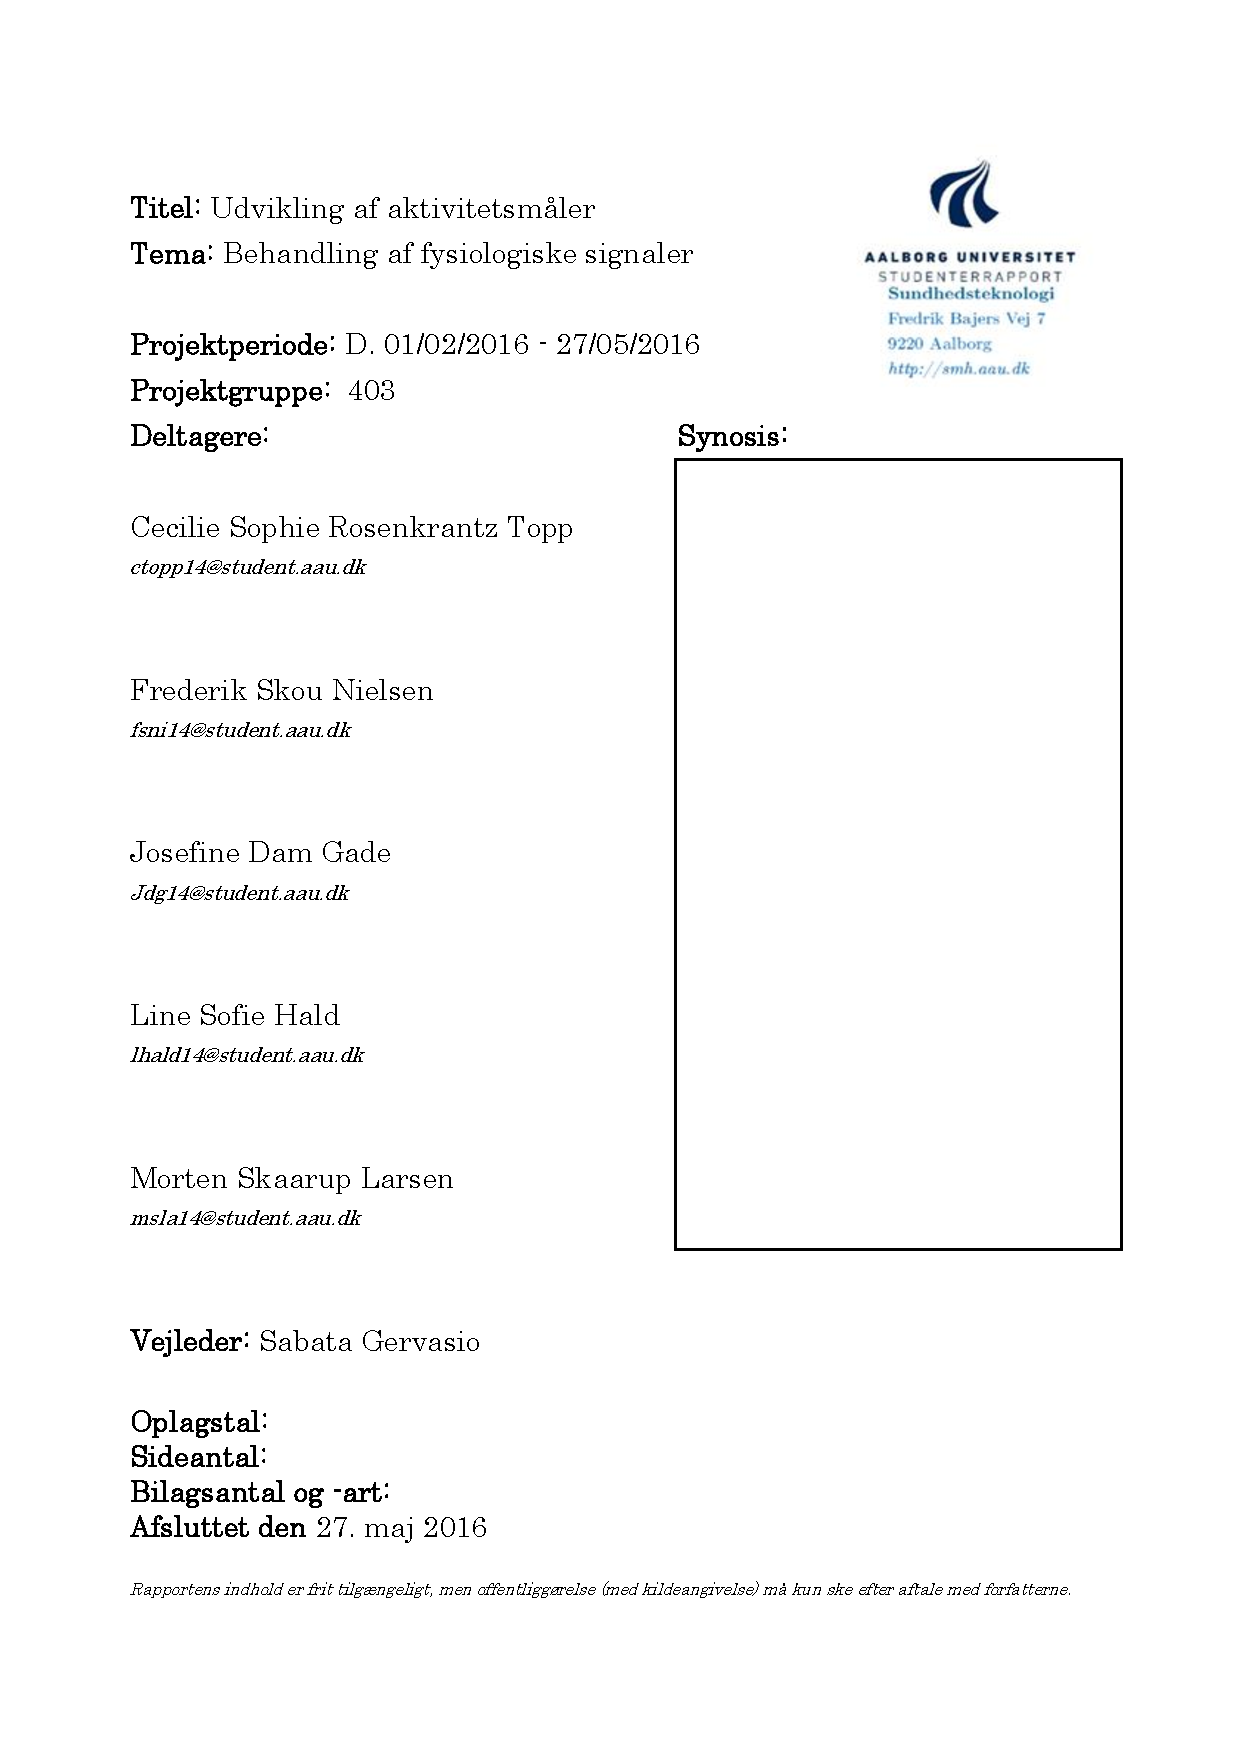
\includepdf[pages={1}]{rapportAfsnit/pFormaliteter/synopsis.pdf} \clearpage 
%\include{rapportAfsnit/pFormaliteter/titelblad}

%\chapter*{Forord og læsevejledning}\vspace{-.75cm}
%% !TeX spellcheck = da_DK
\section*{Forord}
Denne rapport er udarbejdet som et 4. semesters projekt på bacheloruddannelsen i Sundhedsteknologi på Aalborg Universitet. Projektetperioden forløb fra 1. februar 2016 til 27. maj 2016. \\
Projektet tager udgangspunkt i studieordningen for bacheloruddannelsen i Sundhedsteknologi. Semesterets fokusområde er 'Behandling af fysiologiske signaler', hvor dette projekt tager udgangspunkt i projektforslaget 'Udvikling af aktivitetsmåler'. Formålet er blandt andet design, implementering og test af en prototype, der kan detektere fysisk aktivitet. Protoypen udvikles med henblik på at bestemme det fysiske aktivitetsniveau for børn i aldersgruppen 9-12 år. %Prototypen vil derfor involvere en dataopsamling fra analoge komponenter i form af et et accelerometer, et gyroskop og en pulssensor. Ydermere vil prototypen indeholde signal- og databehandling som muligøre digital visualisering på et grafisk brugerinterface.

%Projektet henvender sig til studerende på samme niveau eller andre interessere med et kendskab til basal analog og digital databehandling. \\
Der rettes en tak til vejleder Sabata Gervasio for et godt og lærerigt samarbejde under udarbejdelsen af denne rapport. Yderligere rettes der en tak til semesterkoordinater, John Hansen, for råd og vejledning til forståelse af semesterets nye mikrokontroller. 

\section*{Læsevejledning}
Projektet er opbygget af fem kapitler, en litteraturoversigt samt to bilag. Hvert kapitel og hovedafsnit indledes med et kursiv afsnit, som har til formål at vejlede læseren i henholdsvis kapitlets og hovedafsnittets indhold og sammenhæng i rapportens helhed.\\
Første kapitel består af en indledning og initierende problemstilling. Herefter er problemanalysen, der bearbejder den initierende problemstilling, hvilket leder frem til en problemformulering. Det tredje kapitel er problemløsning, hvori løsningsstrategi og essentielle teoretiske elementer beskrives. Yderligere indeholder kapitlet krav til prototypen og dets delelementer. Det efterfølgende kapitel består af design, implementering og test af systemets delementer samt en test af det samlede system. Afslutningsvis findes syntesen, indeholdende diskussion, konklusion og perspektivering.

Rapporten benytter Vancouver metoden til kildehenvisning. Alle benyttede kilder er at finde på side 91, hvor de er listet i numerisk rækkefølge. I tilfælde, hvor kilden befinder sig inden for punktum, tilhører denne kildehenvisning indholdet i den pågældende sætning. Er kildehenvisningen placeret efter punktummet i sætningen, tilhører kilden indholdet i det foregående afsnit. \\
Tabeller og figurer er nummereret efter deres respektive afsnit, hvorfor eksempelvis figur 1.1 er den første figur i kapitel 1.

Rapporten benytter forkortelser, hvor ordet skrives ud første gang det præsenteres med tilhørende forkortelse i parentes efter ordet. Efterfølgende vil denne forkortelse blive benyttet i resten af rapporten med undtagelse af overskrifter. 
%\newpage

%the '*' allows the tableofcontents be excepted from the actual table of contents.
\tableofcontents* 

%numbers the pages with Arabic numeral - starts from 1.
\mainmatter

\chapter{Introduktion}\vspace{-.75cm}
Artrose, eller slidgigt i daglig tale, er den mest udbredte gigtsygdom der findes. Derudover er den en af de mest udbredte kroniske sygdomme i Danmark [3]. Denne sygdom er en kronisk ledsygdom der kan ramme alle ledstrukturer, dog rammer den primært ledfladernes bruskdele[2] 
Typiske kendetegn ved denne sygdom er smerter, herunder belastningssmerter, og i nogle tilfælde hvilesmerter, ømhed og ledstivhed  [2]. Sekundært påvirkes senerne og muskulaturene ved det afficerede led, og disse forandringer kan føre til et funktionstab. Ved artrose vil håndfunktionen og gangfunktionen være de hyppigst påvirkede funktioner [2]. 
Ifølge spørgeskemabaserede data fra den nationale sundhedsprofil 2013, er prævalensen på 800.000 personer i alt i Danmark. Derudover medfører sygdommen  over 20.000 indlæggelser på årlig basis [3]. Forekomsten af artrose stiger med alderen, hvor det især er de 55-84 årige der er overrepræsenterede. Desuden er der en højere forekomst blandt kvinder end blandt mænd [3]. 
Personer der har et uddannelsesniveau der svarer til grundskole/kort uddannelse, vil også have flere indlæggelser end personer der har en mellemlang/lang uddannelse. Overvægt, tidligere skader, muskelsvaghed, arvelige anlæg mm. spiller også en væsentlig rolle i udviklingen af artrose [3]. Den øgede gennemsnitlige levealder sammenholdt med en øget forekomst af overvægt, vil sandsynligvis medføre at  forekomsten af artrose vil stige i fremtiden. Derudover kan det nævnes at artrose er årsag til 3,2\% af alle tilkendelser af førtidspensioner i Danmark[3].
En af de hyppigst forekommende artroseformer er knæartrose. Denne afgrening af artrose er den førende årsag til funktionsnedsættelse i de nedre ekstremiteter [5]. Kigger man på gruppen af de 60-70 årige har 40\% af kvinderne og 25\% af mændene artrose i knæleddet [2].
Hele knæleddet rammes og er patofysiologisk karakteriseret ved gradvist fremadskridende destruktion af ledbrusken, ledsaget af reaktioner i knoglen under brusken og synovialmembranen [1]. Som følge af den tiltagende bruskmangel kan der opstå ledskurren og fejlsstilling, hvilket kan medføre belastningssmerter og i sidste ende funktionstab [10].  
Der er stor variation i hvordan personer der lever med denne sygdom påvirkes, og nogle vil derfor kunne leve relativt upåvirkede med sygdommen, mens andre vil opleve at sygdommen svækker både arbejdsevne og livskvalitet [3]. Derudover forekommer der kun i ringe grad sammenhæng mellem røntgenfund og patientens oplevede symptomer, og derfor vil behandlingen ofte bero på en vurdering af begge dele [2].
Artrose kan ikke helbredes, men medicinsk behandling vil søge at dæmpe smerter der er forbundet med sygdommen, samt at forbedre funktionen af det afficerede led. Behandlingen af knæartrose afhænger af sværhedsgraden af artrosen, samt patientens alder og situation. I lette og moderate tilfælde er behandlingen altovervejende non-operativ. I disse tilfælde vil fokus være på træning, livsstilsomlægning og patientuddannelse[2].
Ved svære artrosetilfælde, hvor artrosen er radiologisk eller artroskopisk påvist, kan knæalloplastik være en mulighed. Her vil det dreje sig om en individuel vurdering af patientens gener kontra de ricisi der er forbundet med et operativ indgreb [2]. Dog bør behandling af knæartrose altid indledes med non-operativ behandling.


Knæalloplastik, som er en samlebetegnelse over total knæalloplastik (TKA) og unikompartmental knæalloplastik, er indgreb hvor patienten får udskiftet knæleddet enten helt eller delvist. Der er sket en stigning af disse operationer fra 2.500 i år 2000, til over 9000 i år 2015 [12].  I næsten 90\% af alle tilfælde vil alloplastiken være en TKA [10] [12].
For patienter der har gennemgået en ellers succesfuld operation, vil omtrent 20\% opleve kroniske smerter et år efter operationen [11]. Fra et patientperspektiv kan operationen derfor betragtes som en risikabel satsning, hvorfor det er relevant fortsat at søge at forbedre henholdsvis behandling og forståelse for patienternes egne forudsætninger for et vellykket behandlingsforløb. 

\chapter{Problemanalyse}\vspace{-.75cm}
\section{Patientgruppe}
\textit{Følgende afsnit omhandler omfanget af lidelsen, knæartrose. Afsnittet redegør for patientomfanget, samt de forskellige disponeringsfaktorer, sammenkoblet med lidelsen. Ydermere vil patienternes patientforløb blive redegjort, hvoraf den sidste fase vil blive analyseret. Ovenstående vil danne grundlag for at klassificere en disponeret patientgruppe til knæalloplastik.}

Knæartrose er en lidelse hvor primært knæets ledbrusk gradvist bliver nedbrudt, og der sekundært sker forandringer i leddets knogler. Disse deformationer er irreversible, og kan dermed kan knæartrose kun afhjælpes og ikke kurreres. Lidelsen kan opdeles i en primær- og sekundær artrose. Dette adskilles per definition ved at den sekundære artrose indebærer tidligere skader, sygdom, inflammation, overvægt samt traume. Knæartrose er en tilstand hvis hyppigste symptomer indebærer smerter samt nedsat mobilitet hos den udsatte. Smerterne udtrykkes i forskellig grad, fra led igangsættende smerte til kronisk tilstedeværende smerte. Generelt for knæartrose, så forværres symptomerne i takt med graden af lidelsen øges. [Lægehåndbog, knæartrose]

Forekomsten af knæartrose er sammenholdt med en længere række faktorer, hvoraf man er i risiko for at være disponeret. Dette omhandler eksempelvis, overbelastning igennem arbejde og fritid, tidligere knæskader, arv, overvægt samt køn(kvinder)[Knæartrose – nationale kliniske retningslinjer, Sundhedsstyrrelsen]. Knæartrose er tilstede blandt 45\% af alle 80-årige blandt befolkningen. Dette tilfælde kan formodes at stige, som resultat af at der ses en tendens i samfundet, at levealderen i Danmark stiger. Dette er ikke det eneste tilfælde hvorfor prævalensen vil stige. En af de disponerende faktorer for knæartrose er overvægt, hvilket 47\% af den danske befolkning kan kategoriseres under. Ydermere stiger forekomsten af overvægt med alderen, hvilket forud for overvægten ligeledes er tilfældet for knæartrose. Overvægtige er disponeret for knæartrose med en relativ risiko på tre, hvoraf en kombination af ovenstående faktorer øger risikoen for lidelsen. [Patienthåndbogen, overvægt og fedme][lægehåndbog, overvægt][Patienthåndbog, slidgigt i knæ][Lægehåndbog, knæartrose]

Resultatet af en patients komplikationer kan medføre igangsættelse af et behandlingsforløb. Et behandlingsforløb for en patient med knæartrose består af flere faser, hvis mål er smertelindrende, mobilitetsforøgelse samt forebyggende. Generelt kan faserne opdeles i ikke-invasive og invasive metoder. Hvilken metode som afhjælper patienten afhænger heraf af graden af knæartrose. Første fase, hvis nødvendig, består af i en livsstilsændring, hvor en vægtreduktion samt øget fysiskaktivitet uden belastning, vil være fordelagtigt. Hvis dette ikke er tilstrækkeligt kan medicinsk behandling i form af smertelindrende medikamenter benyttes, enten som enkeltstående behandling eller sideløbende med fysioterapi. Hvis ikke, de ikke-invasive behandlingsmetoder afhjælper lidelsen i en grad hvor patienten er tilfreds, så bliver de invasive behandlingsmetoder taget til overvejelse. Overvejelsen heraf indebærer af den diagnosticerede grad af artrose, hvilket består af en sammenkobling af den kliniske vurdering, verificeret med forandringer i knæet opnået gennem røntgenbilleder. Baggrunden for at den kliniske vurdering skal verificeres forud for kirurgi, er at smerte fra hofte og ryg, kan projiceres til knæet.\\
Resultatet heraf er at patienten skal besidde svær slidgigt før patienten kvalificeres til kirurgi, og hermed en total knæalloplastik (TKA).  [Lægehåndbog, knæartrose][Knæartrose – nationale kliniske retningslinjer, Sundhedsstyrrelsen]

TKA er det sidst mulige behandlingsmetode for at udrede patientens komplikationer vedrørende knæartrose. Dette resulterede i at der i 2014 blev udført omtrent 9,8 tusinde TKA operationer, fordelt på førstegangs- og revisions operationer. [Dansk knæalloplastikregister, 2015] I takt med at TKA er den sidst mulige behandlingsmulighed, er operationstilfredshed en betydningsfuld problematik. I 2012 var 81-85\% af patienter der havde modtaget en TKA operation tilfredse, 8-11\%var decideret utilfredse, og resten var i tvivl eller til dels utilfreds. Dette er altså ensbetydende med at der potentielt er 19\% af alle operationer fra et patientøjemed som er ikke succesfulde. Resultatet heraf er at op mod 19\% ikke kan udredes fra deres smerter samt eventuel nedsatte mobilitet, trods alle behandlingsmetoder har været benyttet. [Knæartrose – nationale kliniske retningslinjer, Sundhedsstyrrelsen] Studiet af xxxxx har lavet en risikovurdering vedrørende kroniske smerter postoperativ TKA. Resultaterne betød at op mod 39\% af studiets patienter oplevede moderat til alvorlig smerte, 1 år postoperativt TKA. Ifølge International Association of Pain (IASP) er der tale om kroniske smerte, da dette er tilfældet ved vedvarende smerter tre måneder postoperativ. [Risk Assessment for Chronic Pain,link]. \\
Patientgruppen som postoperativt ikke er tilfredse er svært definerbar. Problematikken opstår i og med klassificeringen bag de potentielt 19-39\% udtilfredse patienter er vedrørende postoperative smerte samt mobilitet. Det kan forestilles at der blandt patienterne en forventningsfaktor, hvilket gør de kategoriserer dem selv som værende utilfreds, omend de rent faktisk har opnået en forbedring af både smerte og eller mobilitet. Det kan tænkes at forventningsfaktoren kan være medvirkende til kategorisere dem som værende utilfredse, som resultat af skuffelsen af ikke at fungere som et individ med et fuldt funktionsdygtigt knæ.  

Knæartrose er på bekostning af samfundets udvikling, en lidelse i vækst da den umiddelbare disponerede målgruppe er voksende. Resultatet heraf medfører at antallet af registrerede tilfælde vedrørende komplikationer sandsynligvis ligeledes vil stige, og der vil forekommer flere patienter med kroniske smerter postoperativt TKA, uden mulighed for yderligere alternativ behandling.


\textit{Kilderne er ikke sat ind - forstår stadig ikke mendeley. Når jeg opretter en manuel kilde - feks. web article, så kan jeg ikke vælge/se nogle citation key.}


\section{Behandling}
Behandlingsforløbet af en patient med knæartrose indeholder flere komponenter, og kan både være kirurgiske og non-kirurgiske alt afhængt af graden af artrose.
\subsection*{Knæledet}
Knæet, \textit{articulatio genus}, er et synovialt, sammensat led med en bevægelsesgrad fra 0 til 135$\degree$ fleksion til 0 til 5$\degree$ ekstension. Knæleddet er legemets største led, hvormed det også er udsat for større mekaniske påvirkninger end noget andet led i kroppen. Hermed er knæleddet hyppigere end noget andet led sæde for patologiske forandringer. Knæleddet er sammensat af tre dele; \textit{femur}, \textit{tibia} og \textit{patella}. Disse er alle i slidfladerne beklædt med et tykt lag hyalinbrusk, op til syv millimeter på femur. Sammen med meniskerne, der fordeler trykket på en større overflade, er hyalinbrusken med til at mindske friktionen i leddet. [\textbf{(Bevægeapperatets anatomi) <- det skal være en rigtig kilde}]

\begin{figure}[H] 
\begin{center}
\includegraphics[width=0.5\textwidth]{figures/bProblemanalyse/Artose_knae}
\end{center}
\caption{Når det normale knæ undergår patologiskeforandringer ved knæartrose vil strukturne i knæet forandre sig. Brusken kan ved infektion, slid eller traume blive beskadiget, hvilket vil eksponerer knoglen og førere til smerte.\citep{schroder} \citep{adobe}} 
\label{fig:tka_implant} 
\end{figure}

\subsection{Ikke-kiurgisk behandling}

Artrose kan som tidligere nævnt ikke helbredes, og non-kirurgiske behandlingsmetoder vil derfor fortrinsvis søge at smertelindre samt forbedre funktionen af knæet \citep{brostrom2012}. En essentiel del af behandling af knæartrose, består af at informere og uddanne patienten, med henblik på at patienten opnår indsigt i sygdommen, samt at patienten aktiv inddrages i behandlingsforløbet. Herved ønskes det at patienten forstår vigtigheden af et vægttab, i så fald dette er nødvendigt. da dette kan være med til at reducere belastiningen på det afficerede led \citep{brostrom2012}.
Ved behandling af artrose benyttes også medcin af forskellig karakter til smertelindring samt forbedring af funktionen. De benyttede præperater er først og fremmest Parcetamol som  førstevalgspræperat, men også NSAID præparater kunne være gavnligt ved inflammation \citep{schroder}. Ved kraftige smertegener, hvor anden smertelindrende behandling ikke har haft den ønskede smertelindring, kan opioider også benyttes. Derudover findes andre medikamenter, som for eksempel steroidinjektioner og glucosamin præparater. Derudover benyttes også ganghjælpemidler og skinner. Disse benyttes dog i et mindre omfang \citep{brostrom2012}.\\

I behandlingsforløbet er træning en vigtig faktor, både før og efter en eventuel operationen. Dette afspejles i både nationale og internationale kliniske retningslinjer, hvor der er bred konsensus om, at træning er af væsentlig betydning ved behandling af knæartrose \citep{brostrom2012}. Et systematisk review med data fra over 4000 patienter, foretaget af \cite{Syssorenskou}, viste at hverken graden af den røntgenpåviste artrose eller smerteintensitet havde indvirkning på hvor stor effekt der kunne forventes af træningsforløbet. Det blev fundet at patienter med svær artrose oplevede samme smertereduktion som patienter med let til moderat artrose efter træningsforløbet. Et Cochranereview finder evidens for at den forventede smertelindring ved træning er lige så stor som ved brug af NSAID og endnu større end ved brug af parvetamol. Træning har ligeledes den fordel ikke at have bivirkninger som smertelindrende medicin har \citep{sorenskou}.
I et dansk studie, der strakte sig over 12 måneder blev 100 patienter  der var egnet til at modtage en TKA, randomiseret i to grupper. Den ene gruppe skulle modtage non-kirurgisk behandling som bestod af et træningsforløb, patientundervisning, indlægssåler og et eventuel vægtabsprogram. Den anden gruppe modtog kirurgisk behandling efterfulgt af et non-invasivt forløb. Gruppen der gennemgik kirurgisk behandling efterfulgt af et non-invasivt forløb, havde en større smertelindring en gruppen, som kun modtog ikke-kirugisk behandling. Dog havde gruppen der modtog kirurgisk behandling større risiko for at få alvorlige komplikationer. Forsøget viste desuden at i gruppen som skulle modtage non-kirurgisk behandling, fik over to tredjedele ikke foretaget en TKA inden de 12 måneder \citep{newEngland}. 

%Dette kan muligvis betyde at et non-invasivt forløb kan være være med til udskyde et operativt indgreb. (\textbf{vi skal nok passe på med at konkludere noget her})

%\subsection{Knæartrose}
%
%Knæartrose også kaldet slidgigt i knæene, har mange årsager. Hvor af nogle er overvægt, arv, traume eller tungt arbejde. Arterose er karakteriseret ved ødelæggelse af ledbrusken med dertil hørende reaktioner i de tillæggende knogler og slimhinder. Symptomerne på knæartrose er smerte, funktionstab og fejlstilling, hvilket besværliggøre hverdagen. 
%Ved knæartrose er sidste behandlings skridt kirurgi, afhængig af graden af traumet er forskellige kirurgiske indgreb en mulighed. [Nationale retningslinjer] 

\subsection{Kirurgisk behandling}

Når de non-kirurgiske behandlingsmuligheder ikke har kunne løse patienten fra smerter, er kirurgi det næste skridt i behandlingsforløbet. Der findes flere behandlingsmuligheder inden for kirurgiskbehandling af artrose. Valget af operation og typen af den afhænger af flere faktorer, blandt andet patients alder, aktivitetsniveau og hvor fremskreden artrosen er.

\subsubsection{Osteotomi}
Ved degenerative forandringer i knæleddet, grundet primær eller postttrumatisk knæledsarterose, kan patienter opleve belastningsreleaterede smerter, hvilket blandt andet kan skyldes fejlstilling. Osteotomi har tilformål at afhjælpe den mekaniske belastning i det berørte område, for derved at afhjælpe smerterne. Ved osteotomi fjernes der oftest en kile af tibia-knoglen og det resterende knogle sikres med skruer og metal plader. Proceduren ændre knæets mekaniske akse, hvilket vil ændre belastningen af de degenererede områder. \citep{Osteotomi_og_TKA} Ved yngre (<50år) og aktive patienter vil der være større sandsynelighed for at tilbyde osteotomi frem for den mere invasive TKA, derfor anbefales osteotomi af sundhedstyrelsen til behandling af mildere former for artrose med fejlstilling \citep{Osteotomi_og_TKA} \citep{brostrom2012}. Behandlingen ses som en midlertidig behandling der kan udskyde behovet for TKA. Ifølge et kohordestudie kan der forventes en smertelindring hos 80\%~ af patienterne der får udført osteotomi. \textbf{rigtige kilder tak!(79)(80)} Ifølge \cite{brostrom2012} må det forventes at 30 til 50\%~ af patienterne der får foretaget en osteotomi, senere vil få behov for en alloplastik operation. \citep{brostrom2012} Tilbagevendende smerter korreleres til tab af korrektionen, samt progression af artrosen. Får patienten således svære smerte igen, kan en TKA komme til overvejelse \citep{Osteotomi_og_TKA}. 
% \textbf{Der er data på mere specifikke tilfredsheds undersøgelser, men ser ikke nogen trund til at medtage dem. }

\subsubsection{Alloplastik}
Alloplastik er et operativt indgreb der har til formål helt eller delvist at udskifte knæleddet, med specielt designede metal- og plastkomponenter som varig erstatning for bruskfladerne i knæet. Operationen opdeles i TKA og UKA, hvilket henholdsvis er helt eller delvis udskiftning af knæleddet og afhænger af den specifikke diagnose. Der kan ved traume tilfælde eller svære beskadigelser af de anatomiske strukturer omkring knæet forekomme specialiserede udgaver af knæalloplastik.

\begin{figure}[H] 
\begin{center}
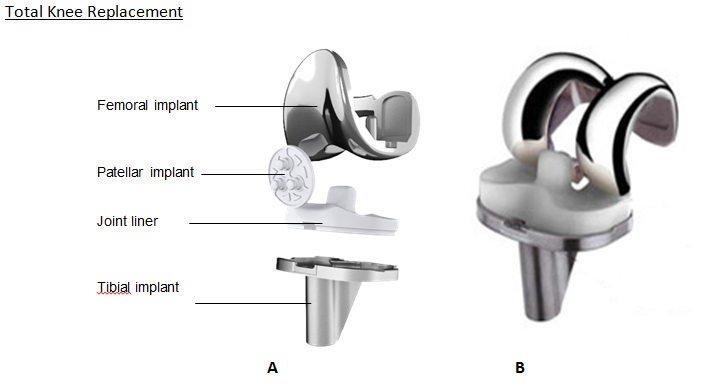
\includegraphics[width=0.7\textwidth]{figures/tka_implant}
\end{center}
\caption{Komponenterne til en total knæalloplastik, består af et femural og tibia implantat ofte bestående af en titaniumlegering. Patella- og tibiaindsatsen er lavet af polyethylen, hvilket er med til at mindske friktionen og efterligne knæledes naturlige bevægelse.\cite{1}} 
\label{fig:tka_implant} 
\end{figure}

Under selve operationen ligger patienten supineret på operationsbordet med knæet i en flekteret position. Et longitudinelt snit lægges over midten af patella. Patella og senerne eleveres og blotter knæleddet, hvilket giver kirurgen adgang til bruskfladerne på femur og tibia. Herefter fjerner kirurgen det ødelagte brusk, ved hjælp af en guideblok der skrues ind i femur og sikrer præcis fjernelse af den ønskede mængde væv. Dette gentages på tibia, hvorved der skabes plads til implantaterne. Midlertidige implantater indsættes for at sikre bevægelsesfriheden er bevaret og testes ved ekstension af knæet for at sikre at den rigtige mænge brusk og knogle materiale er fjernet. Når kirurgen er tilfreds med resultatet bores der guidehuller i henholdsvis femur, tibia og patella til fastemontering af de permanente implantater. Fastmontering sker ved at dække implantatet og monteringsstedet i bencement der limer proteserne fast til den eksisterende knogle struktur. Herefter sikres endnu engang at bevægelsesgraden er bibeholdt, førend indsnittet lukkes og operationen er fuldendt. En TKA operation varer typisk omkring én time, hvorefter patienten kan støtte på benet den følgende dag. Efter operationen følger et rehabiliteringsforløb for at støtte og styrke muskulaturen omkring knæet. \citep{Sanna2013} \citep{tka-technique}

Ifølge sundhedsstyrelsens vurdering er knæalloplastik, effektiv til at mindske smerte, øge funktion og derved bedre livskvalitet. Holdbarheden af knæimplantaterne vurderes ud fra antallet af implantater der er blevet udskiftet efter 10 år, hvor det findes at 90 til 95\%~ af implantaterne ikke er revideret. Dog skal det nævnes at det ikke er muligt at vurdere holdbarheden af den enkelte protese, da flertallet af patienter dør med en velfungerende implantat. \citep{brostrom2012}

\paragraph{Succeskriterier}

Succeskriterier for kirurgisk behandlingen af arterose er ifølge styrringsgruppen for Dansk knæalloplastikregister (DKA) \citep{aarsrapport2016} opdelt i fem kriterier.
%, som alle bygger revisionsraten. Altså patienter som har behov for en yderligere knæ operation.  

% Please add the following required packages to your document preamble:
% \usepackage{graphicx}
% \usepackage[table,xcdraw]{xcolor}
% If you use beamer only pass "xcolor=table" option, i.e. \documentclass[xcolor=table]{beamer}
\begin{table}[H]
\centering
\caption{Tabellen viser succeskriterierne for knæalloplastikoperationer med en standard acceptabel grænse sammenholdt med landsgennemsnittet. Spredning er indikeret i parentes. Tabellen er modificeret fra \citep{aarsrapport2016} }
\label{succeskriterier}
\resizebox{\textwidth}{!}{%
\begin{tabular}{lcc}
\hline
\rowcolor[HTML]{C0C0C0} 
Indikator                                                                                                                                                                                                                                                  & Standard    & \begin{tabular}[c]{@{}c@{}}Landsgennemsnit\\ (Spredning)\end{tabular} \\ \hline
\begin{tabular}[c]{@{}l@{}}\textbf{Genindlæggelse}\\ \\ Andel af alle patienter med primær knæalloplastik på baggrund af primær artrose, \\ der genindlægges uanset diagnose indenfor 30 dage efter udskrivning\end{tabular}                                        & Højest 10\% & 7,3 \% (5,8-9,5)                                                      \\ \\
\begin{tabular}[c]{@{}l@{}}\textbf{Revisionsrate det første postoperative år}\\ \\ Andel af alle patienter med primær knæalloplastik fra et givent operationsår, \\ der er revideret (dvs. implantat fjernes, udskiftes eller tilføjes) indenfor 1 år.\end{tabular} & Højest 3\%  & 1,8 \% (0,8-2,4)                                                      \\ \\
\begin{tabular}[c]{@{}l@{}}\textbf{Revisionsrate de første 2 postoperative år}\\ \\ Andel af alle patienter med primær knæalloplastik fra et givent operationsår, \\ der er revideret (dvs. implantat fjernes eller udskiftes) indenfor 2 år.\end{tabular}          & Højest 5\%  & 3.3\% (1,7-4,8)                                                       \\ \\
\begin{tabular}[c]{@{}l@{}}\textbf{Revisionsrate de første 5 postoperative år}\\ \\ Andel af alle patienter med primær knæalloplastik fra et givent operationsår, \\ der er revideret (dvs. implantat fjernes, udskiftes eller tilføjes) indenfor 5 år.\end{tabular}   & Højest 8\%  & 6,0\% (4,2-6,7)                                                       \\ \\
\begin{tabular}[c]{@{}l@{}}\textbf{Mortalitet indenfor 90 dage}\\ \\ Andel af patienter, der dør indenfor 90 dage efter primær knæalloplastik.\end{tabular}                                                                                                         & Højest 1\%  & 0,4\% (0,0-0,7)                                                      
\end{tabular}%
}
\end{table}

Som det ses af \tabref{succeskriterier} udføres der i hele Danmark knæoperationer som alle signifikant overholder indikationerne for behandlingskvaliteten \citep{aarsrapport2016}. 
På trods af at alle operationer overholder succeskriterier, ses det at patienter postoperativt har smerter og er utilfredse. Antallet af patienter på tværs af studier som er utilfredse er 11 til 25\%, se \tavref{patient_utilfreds} (n=31.114) hvoraf studiet med størst deltagelse (n=27.372) viste at 18\%~ af patienterne var utilfredse. \citep{Bourne2010}

Studiet af \cite{Sakellariou2016} rapporterer postoperative smerter hos patienter, hvor 39\%~(n=272) oplevede moderat til alvorlige smerte\citep{Sakellariou2016}. Et andet studie viste at 19\%~ af patienterne havde svære til uudholdelige smerter efter den første operation. Ved revision var procentdelen af patienter med svære til uudholdelige smerter 47\%. \citep{Petersen2015}

Patienterne burde efter operationen være tilfredse samt smertefri, dette er imidlertid ikke tilfældet. Der er således et problem med resultatet af operationen, på trods af operationen overholder succeskriterierne \citep{aarsrapport2016}. Det må derfor antages problemet ikke ligger ved operationen, men da en del patienter oplever postoperative smerter, er det relevant at undersøge smertes indflydelse på resultatet af operationen. 

%
%(1) http://www.robodoc.com/patient_about_faqs.html
%
%(2) https://www.youtube.com/watch?v=tKji04oFGdU

% (3) http://www.ortopaedi.dk/fileadmin/Guidelines/Referenceprogrammer/Osteotomi_og_TKA.pdf

	%(4) Surgical approaches in total knee arthroplasty.
	
%	(5) tka-technique
%
%(79) Dahl AW, Toksvig-Larsen S, Roos EM. A 2-year prospective study of patient- relevant outcomes in patients operated on for knee osteoarthritis with tibial osteot- omy. BMC Musculoskeletal Disorders 2005;6(1):18. Er lagt på mendlay
%(80) Hoell S, Suttmoeller J, Stoll V, Fuchs S, Gosheger G. The high tibial osteoto- my, open versus closed wedge, a comparison of methods in 108 patients. Arch Or- thop Trauma Surg 2005;125(9):638-643. Er lagt på mendelay
\section{Smerte}

Smerte er blevet defineret som: “en ubehagelig sensorisk og emotionel oplevelse forbundet med egentligt eller potentiel skade af væv eller beskrevet i vendinger tilsvarende en lignende skade.” af den Internationale Association for Studiet af Smerte (Pain) (IASP) [Seminars in arthritis and rheumatism, Classification of Chronic Pain]. 
Selvom smerte normalt er en følelse man forsøger at undgå, er det en nødvendig del af vores overlevelse. Det fortæller kroppen om farer eller skader som der skal reageres på, som for eksempel at sætte hånden på en varm kogeplade. For ikke at blive slemt forbrændt og gøre skade på hånden, registrere nerver i huden en høj temperatur, som hånden skal fjernes fra. Nervesignalet sendes til central nervesystemet (CNS), hvor det først når rygmarven og lidt senere hjernen. Her skelnes der mellem smerte sensation og perception. Smerte sensation er information om smerte, som nerverne i hånden der registrere den skadelige temperatur. Smerte perceptionen sker først når nervesignalet når op til hjernen og denne modtager signalet og opfatter det som smerte. Sensationen af smerte kan i rygsøjlen aktivere en refleks der får musklerne i armen til at trække hånden væk fra varmen, inden hjernen når at registrere og opfatte den egentlige smerte. [Fundamentals of Human Anatomy and Physiologi 9th edition] Denne form for smerte er kategoriseret som øjeblikkelig smerte og defineres som “god” eller “nødvendig” smerte, da det hjælper kroppen med at undgå skader.

\subsection{Smerte typer}
Modsat denne “gode” smerte findes “dårlig” eller “unødvendig” smerte. Denne smerte kaldes også kronisk smerte, da den oftest er længere varende, ved at have været mere eller mindre konstant i mindst tre måneder [Seminars in arthritis and rheumatism]. Personer som lider af kronisk smerte har sjældent en synlig grund til at skulle føle smerte, og smerten er af den grund enten oplevet som smerte i indre organer eller psykogene smerter, som er forestillingen om en smerte. 
Ved organisk smerte skelnes der mellem to typer af smerte: nociceptisk og neuropatisk. Nociceptisksmerte er skade på væv og skyldes aktivering af nociceptorer, specielle nerveceller som er følsomme overfor temperatur ændringer, mekanisk stimuli eller kemiske ændringer i eller omkring celler, ved hjælp af specielle porte og pumper på nervecellerne. Nociceptorer findes i huden på kroppens overflader og i og omkring indre organer, og nociceptisksmerte opdeles i somatisk og viseral sensation. Somatisk smerte sensation og den øjeblikkelige og let placerbare smerte som at sætte hånden på en kogeplade. Viseral smerte sensation er mere besværlig at placere. Smerten er typisk ikke øjeblikkelig, men mere trykkende og langvarig. At have ondt i maven er et eksempel på viseral smerte. Nociceptisksmerte er oftest ikke årsag til kroniske smerter, med mindre smerterne bliver ved. 
Neuropatisk smerte er modsat nociceptisksmerte ikke skade på væv, men på nervesystemet selv, herunder nerver, rygmarv, nerve plexus eller hjernen. Dette kan skyldes direkte skade, sygdom som iskæmi eller sclerose, traume, diabetes, infektioner eller kræft. Smerten kan opleves som konstant og langvarig, hvor er typisk eksempel er fantom smerter, men kan også være lejlighedsvis som ved hyperalgesi, hvor almindelig berøring opfattes som smertefuldt. [Seminars in arthritis and rheumatism, Classification of Chronic Pain] 
Psykogene smerter er en forestillet opfattelse af smerte, og den mest besværlige at præcisere, idet der ikke er og muligvis aldrig har været en fysisk grund til smerten. Hos en person med psykogene smerter er hjernen fuldt overbevidst om, at den oplever fysiske smerter og lider der af. Smerten er udelukkende psykisk hos personen, men er af den grund ikke mindre virkelig, grundet smertes subjektive natur. [Seminars in arthritis and rheumatism]

\subsection{Problemet ved kronisk smerte og operationer}
Der findes således flere forskellige former for smerte, hvor kun nogle få er beskrevet her [Classification of Chronic Pain]. Alle kan de lede til kronisk smerte. Man ved derfor godt hvad der kan give kronisk smerte, hvordan smerten opfattes og hvor i kroppen den kommer fra. Men man ved endnu ikke hvorfor kronisk smerte opstår. Hvorfor føler kroppen fantom smerter fra et legeme som ikke er der? Hvorfor registrere hjernen smerte fra indre organer, når der intet er i vejen med dem? Et større problem opstår når man forsøger at behandle smerterne, med et ønske om at dæmpe eller helt fjerne smerterne, men smerterne fortsætter eller forværres. Sådan ses det i 20\% af tilfælde efter total knæalloplastik (TKA) operationer [Chronic Postoperative Pain After Primary and Revision Total Knee Arthroplasty]. Her oplever 19\% af patienter efter den primære operation, og 47\% af patienter efter revision af operationen oplever svære til uudholdelige smerter. Dette sker på trods af at der i hele Danmark udføres knæoperationer som alle signifikant overholder indikationerne for behandlingskvaliteten [Dansk Knæalloplastikregister, Årsrapport 2016]. De udførte TKA operationer må siges at være nær perfekte, men patienter oplever alligevel fortsatte smerter. 


\section{Klinisk udvælgelse af patienter}\label{kliniskudvaelgelse}
\textit{I dette afsnit undersøges det hvilke retningslinjer og faktorer, der har betydning for en klinikers henvisning af en patient til en TKA-operation. Dette gøres med henblik på en identifikation af eventuelle problematikker ved en udvælgelse af patienter, som hovedsageligt er baseret på en klinikers vurdering.}

Patienter, som tilbydes en TKA-operation, udvælges på baggrund af en klinikerens observationer og erfaringer. Hermed afhænger udvælgelsen af patienter til en TKA-operation af klinikere, hvormed patienter kan opleve varierende anbefalinger og behandlingsmuligheder afhængig af hvilken kliniker, der er ansvarlig for vurderingen. I et forsøg på at standardisere behandlingen af knæartrose for alle patienter i Danmark har Sundhedsstyrelsen udarbejdet en rapport indeholdende nationale kliniske retningslinjer. Disse retningslinjer bygger hovedsageligt på lægelig konsensus. Retningslinjerne vedrørende tilbud om en TKA-operation indeholder blandt andet, at patienter kun tilbydes en TKA-operation hvis non-invasive behandlingsmetoder ikke har en tilstrækkelig virkning. En TKA-operation kan tilbydes patienter som den første behandlingsmulighed, hvis klinikeren vurderer, at patientens artrose er så svær, at ingen non-invasive behandlingsmetoder vil have en tilstrækkelig effekt. Dette kan eksempelvis være, hvis patienten har en kraftig fejlstilling af knæet eller svær instabilitet i leddet. \citep{brostrom2012} \\
Sundhedsstyrelsen har ligeledes opstillet en række indikationer, som kan få klinikeren til at vurderer at en patient ikke er egnet til en TKA-operation. Disse indikationer er eksempelvis, hvis der er infektion i knoglen eller leddet, hvis patienten ingen smerter har i leddet eller hvis patienten har en kort forventet levetid. En anden indikator, som kan få en kliniker til at fravælge at operere patienten, er hvis patienten har urealistiske forventninger til operationen. \citep{brostrom2012} I et studie har \citer{tejada2010} vist, at patienter, hvis forventninger til operationen bliver opfyldt, oplever større tilfredshed efter operationen. Ligeledes er det vist, at klinikerens forventninger til en operation påvirker patientens forventninger \citep{tejada2010}. Dette antyder, at klinikere, ved at forklare patienten hvad de kan forvente af operationen, kan være med til at mindske eller helt fjerne faktoren vedrørende urealistiske forventninger. \\
Ud fra et studie af \citer{skou2016} anses flere af de ovennævnte retningslinjer som nogle af de vigtigste overvejelser, når en kliniker skal bestemme, om en patient er egnet til at modtage en TKA. \citer{skou2016} fandt, at klinikeren anser røntgenresultater, smerte i knæet ved udførelse af hverdagsaktiviteter, funktionelle begrænsninger samt utilfredsstillende virkning af non-invasive behandlingsmetoder som de fire vigtigste faktorer for en patients egnethed til en TKA-operation. Det blev af \citer{skou2016} undersøgt om de faktorer, klinikerne mente var de vigtigste for en patients egnethed for en TKA-operation, blev afspejlet i hvilke patienter klinikerne tilbød en TKA-operation. Her blev det fundet, at radiologiske resultater samt funktionelle begrænsninger var betydningsfulde i forhold til patientens egnethed til en TKA-operation. De to andre faktorer, smerte i knæet samt utilfredsstillende non-invasive behandlinger, var ikke drivende for klinikerens vurdering af patientens egnethed til en TKA-operation. Hermed blev der af \citer{skou2016} fundet en uoverensstemmelse mellem hvilke faktorer klinikerne fandt vigtigst i forhold til vurdering af behovet for en TKA-operation og hvilke faktorer de samme klinikere udvalgte patienter ud fra. Denne uoverensstemmelse viser, hvor kompleks udvælgelsesprocessen for en TKA er samt vanskelighederne ved at bestemme hvilke faktorer, der har størst betydning for en klinikers beslutningsprocess. Ud fra resultaterne fra studiet af \citer{skou2016} antydes det, at klinikerne anvender både bevidste og ubevidste faktorer til bestemmelse af patienters egnethed til en TKA-operation. Flere studier har undersøgt hvilke ubevidste faktorer, der kan påvirke en klinikers beslutningstagning. Eksempelvis antyder resultater fra et studie udarbejdet af \citer{borkhoff2008}, at en patients køn har betydning for, om klinikeren tilbyder patienten en TKA eller ej. I dette studie anvendte \citer{borkhoff2008} to standardiserede patienter med moderat knæartrose, som besøgte 71 klinikere, bestående af 38 alment praktiserende læger og 33 ortopædkiruger. Klinikerne, som deltog i studiet, blev ikke informeret om hvem de to standardiserede patienter var. De to standardiserede patienter var ens på alle andre punkter end køn. \citer{borkhoff2008} fandt, at 55\% af ortopædkirugerne kun tilbød den mandlige patient en TKA-operation, mens ingen af ortopædkirugerne kun tilbød den kvindelige patient en TKA-operation. Sandsynligheden hvormed en patient vil få tilbudt en TKA-operation afhænger af flere parametre. Eksempelvis kan patientens kommunikationsmetode have indflydelse på beslutningen vedrørende det efterfølgende behandlingsforløb. \citep{borkhoff2008}

 % Mulige grunde til den fundne bias i studiet af \cite{borkhoff2008} kan være, at størstedelen af klinikerne der deltog i forsøget var mænd. Ud af de 71 klinikere som deltog i forsøget var 59 af disse mænd. Resultaterne fra studiet viser ingen signifikant forskel i andelen af mandlige klinikere som kun tilbød den mandlige patient en TKA, og andelen af kvindelige klinikere som kun tilbød den mandlige patient en TKA. Det kunne dog undersøges om klinikere har tendens til oftere at henvise patienter af deres eget køn til en TKA end patienter af det modsatte køn. Dette kunne være relevant at undersøge da studier har vist forskelle i mænd og kvinders kommunikationsmetoder, hvormed klinikerens eget køn kan have en betydning for hvordan en patients beskrivelse af sygdommen opfattes og dermed vurderes. \citep{street2002}   
% Bemærk at det med den signifikante forskel handler om mænd vælger mænd etc. Der var en signikant forskel vedr. om det kun er mænd der bliver valgt
I en spørgeskemaundersøgelse, hvor ortopædkiruger blev bedt om at vurdere betydningen af en patients køn i forhold til, om de ville henstille patienten til en TKA-operation eller ej, svarede cirka 93~\% af de adspurgte klinikere, at køn ikke ville have nogen betydning for deres vurdering af patienten \citep{wright1995}. Dette kan antyde, at den forskel \citer{borkhoff2008} fandt i deres forsøg, er følge af en ubevidst bias hos klinikerne. Teorien understøttes også af resultaterne fra et studie udarbejdet af \citer{dy2014}, hvor det blev undersøgt, om en patients race og køn ville have betydning for klinikerens vurdering af patienter.\\
I dette studie blev videoer med patienter med svær knæartrose anvendt. Ligesom i studiet af \citer{borkhoff2008} var patienterne kun forskellige i køn og race. \citer{dy2014} fandt ingen forskel på klinikerens vurdering af de fire standardiserede patienter. Forskellen i resultaterne mellem \citer{borkhoff2008} og \citer{dy2014} kan skyldes forskellen i patienternes grad af artrose. Ved patienter med svær artrose forekom ingen bias, mens der ved patienter med moderat artrose blev fundet bias. Dette antyder, at klinikernes bias kun har betydning for patienter, hvor der ikke er klare indikationer på, at patienten bør opereres.\\
I tilfælde hvor der ikke er klare indikationer på, at patienten vil opnå bedring ved en TKA-operation, vil en teknologi, der kan hjælpe klinikeren med at udføre en vurdering uden bias være fordelagtig. Ved anvendelse af en sådan teknologi vil det være muligt at inddrage andre faktorer i udvælgelsen af patienter til TKA-operation. Dette vil eksempelvis kunne gøres ved at anvende en teknologi, som kan hjælpe klinikere med at vurdere patienters risiko for at udvikle kroniske smerter efter TKA-operationen. Hermed vil det være muligt at mindske fordelingen imellem den tekniske succes og den patientmæssig succes ved en TKA-operation.

Set i forhold til de opstillede succeskriterier for en TKA-operation beskrevet i \secref{tek_succes} er stort set alle TKA-operationer succesfulde, mens omkring 80\% af patienterne, der gennemgår en TKA-operation, ikke oplever kroniske smerter. \citep{Sakellariou2016} \citep{Petersen2015} En succesfuld operation kan dermed defineres forskelligt alt efter hvilken synsvinkel, der arbejdes ud fra. Ud fra en patientmæssig synsvinkel defineres en succesfuld TKA-operation som en operation, hvor patienten er tilfreds med resultatet af denne. Ud fra et teknisk perspektiv er en TKA-operation succesfuld, når denne opfylder kravene opstillet af DKA \citep{aarsrapport2016}. Problematikken opstår ved de TKA-operationer, som kun er succesfulde ud fra et teknisk perspektiv. For at mindske andelen af disse vil det være fordelagtigt at finde en teknologi, som hæver antallet af tilfredse patienter uden at sænke antallet af operationer, som opfylder de tekniske krav. Da kronisk smerte er en af de hyppigste årsager til utilfredshed blandt patienter efter en TKA-operation, vil en reduktion i antallet af patienter med kroniske postoperative smerter sænke antallet af utilfredse patienter. \citep{Bourne2010} 

Udfra disse kriterier vil en teknologi, som gør det muligt at identificere hvilke patienter, der er i risikogruppen for at få kroniske smerter efter en TKA-operation, være fordelagtig. Hermed vil en del af de TKA-operationer, som ikke gavner patienten, kunne undgås. De ovenstående kriterier vil potentielt kunne opfyldes af flere forskellige teknologier. En analyse af disse teknologier vil derfor kunne identificere den mest optimale teknologi til præoperativ undersøgelse af patienter, således patienter med risiko for udvikling af kroniske postoperative smerter kan identificeres.


\textit{I denne sektion vil nuværende teknologier til undersøgelse af neural aktivitet blive beskrevet med særlig fokus på anvendelse i forbindelse med undersøgelse af smerteopfattelse. Det økonomiske aspekt vil ligeledes blive analyseret for de enkelte teknologier. Afslutningsvis vil der blive foretaget en sammenligning med henblik på at identificere fordele og ulemper ved de enkelte teknologier.}
\section{Teknologier til vurdering af smerte} % Anden overskrift...
For at understøtte klinikerens vurdering af de enkelte patienter vedrørende henstilling til TKA, kan det overvejes, hvorvidt det vil være hensigtsmæssigt at tilføje en ekstra undersøgelse til patientens udredningsforløb forud for beslutningen herom. Relevante undersøgelser kan eksempelvis være objektive målinger på neural aktivitet i forskellige situationer, samt vurdering af patienternes individuelle respons på forskellige typer af stimuli. Til undersøgelse af aktivitet i encephalon og nervesystemets funktion generelt findes flere forskellige metoder.
  
\subsection{fMRI}
Functional Magnetic Resonance Imaging(fMRI) er en metode til at undersøge aktiviteten i neuronerne i hjernen.
Generelt er MRI en metode til at synliggøre protoner; dermed er det muligt at afbilde kroppens væv, da dette primært er udgjort af hydrogen-atomer, som indeholder netop én proton.     
Ved en MRI-scanning udsættes objektet, eksempelvis en patient, for et eksternt magnetfelt, hvilket medfører, at der opstår et parallelt magnetfelt i objektet. Dermed er det muligt at detektere de tilstedeværende protoner, da deres retning skaber det parallelle magnetfelt i kroppen.\citep{Wals2009} Udgifterne til fMRI omfatter blandt andet indkøb af MRI-scanner samt anvendelse og vedligehold.\fxnote{Er i tvivl om, om dette er nok, men ellers er man nødt til at anvende sider, der sælger MR-scannere, og det er ikke særligt gode kilder... Alternativt kan der sættes ét priseksempel ind på en konkret scanner?} 
Der findes forskellige teknikker til fMRI, hvoraf de fleste anvender Blood Oxygenation Level-Dependent(BOLD) kontrast. Ved anvendelse af denne kontrast, udnyttes det, at der ved aktivitet i hjernens forskellige områder, vil ske en ændring af mængden af ilt i blodet, hvilket påvirker magnetfeltets styrke. Dermed vil det, ved hjælp af kontrastvæsken, være muligt at følge blodgennemstrømningens styrke i hjernens forskellige områder. \citep{Wals2009} 

\subsubsection{Anvendelse til detektion af smerte}
fMRI har i flere studier været anvendt til at undersøge neural aktivitet i forbindelse med knæsmerter.
I et studie af \citep{Parks2012} er det ved hjælp af fMRI blevet undersøgt, hvorvidt der er forskel på oplevelsen af kroniske smerter hos patienter med artrose og på smerter fremkaldt med tryk. Forsøgsdeltagerne var opdelt i en gruppe patienter med artrose i knæet og en gruppe raske individer. \textbf{xxxx} viste at de to grupper oplevede den kunstigt fremkaldte knæsmerte ens; der forekom stort set ingen variationer imellem de to grupper. Derimod viste der sig at være forskel på de kroniske smerter og de kunstigt fremkaldte smerter hos patienterne med artrose. \citep{Parks2012} 
I et andet studie af \citep{Hiramatsu2014} er det undersøgt, hvilke forskelle der forekom i cerebral respons hos en gruppe raske forsøgspersoner og en gruppe forsøgspersoner med kroniske knæsmerter forårsaget af artrose. Begge grupper blev udsat for akut smerte gennem invasive elektroder imens der blev foretaget en fMRI scanning. Studiet viste, at der hos gruppen af patienter med kroniske knæsmerter forekom en højere aktivitet i det dorsolaterale præfrontale cortex end hos gruppen af raske forsøgspersoner. \citep{Hiramatsu2014} 
fMRI kan således påvise forskelle på hvordan smerte opleves af forskellige grupper af mennesker. Figur \ref{fig:fMRI_result} illustrerer forskellen i neural aktivitet mellem patienterne og den raske forsøgsgruppe.
\begin{figure}[H] 
	\begin{center}
		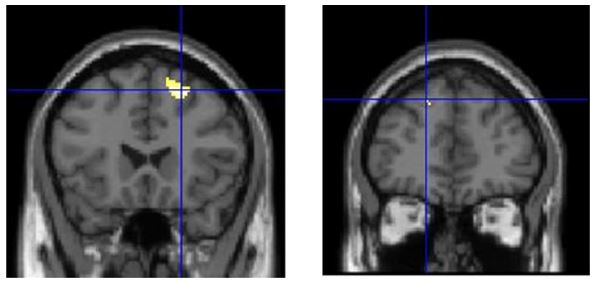
\includegraphics[width=0.7\textwidth]{figures/bProblemanalyse/fMRI_dorsolateral}
	\end{center}
	\caption{Figuren illustrerer forskellen imellem henholdsvis patientgruppen og den raske forsøgsgruppe. Det fremgår, at aktiviteten i det dorsolaterale cortex er signifikant højere hos patienterne end hos de raske individer. \citep{Hiramatsu2014}} 
	\label{fig:fMRI_result} 
\end{figure} 

\subsection{Quantitative sensory testing}
Quantitative sensory testing(QST) er en metode til undersøgelse af det sensoriske nervesystems funktion. Metoden kan anvendes til undersøgelse af forskellige egenskaber, herunder smertegrænser. Ved en QST-undersøgelse eksponeres patienten for forskellig sensorisk sensation, herunder tests, der involverer varme og kulde, vibration og tryk. Dermed er det muligt at identificere grænserne for henholdsvis perception og smerte. \citep{Yarnitsky2006} QST kræver - i modsætning til fMRI - ikke scanning eller anden billeddiagnostisk undersøgelse. 
Der findes forskellige protokoller til QST-undersøgelse, der alle indeholder tests indenfor de forskellige områder, der ønskes undersøgt ved en QST. Et eksempel er en QST-protokol udviklet af German Network on Neuropathic Pain til undersøgelse af neuropatisk smerte. Ved brug af denne model anvendes syv forskellige tests til at vurdere 13 parametre, herunder seks temperaturtests til detektion af grænser for perception og smerte samt syv mekaniske tests til detektion af tilsvarende grænser, her med henholdsvis spidste og stumpe genstande. I forbindelse med udarbejdelse af modellen er der desuden lavet tests for at opstille referenceværdier, der tager højde for både køn og alder. citep{8}  

\subsubsection{Anvendelse til detektion af smerte}
QST bliver i forskningsregi anvendt til undersøgelse af patienter der får udført TKA. I et studie af \citep{Martinez2007} er en anden QST-protokol anvendt til at undersøge 20 patienter med artrose i knæet før og efter en TKA. Formålet hermed var at identificere faktorer, der har indvirkning på udviklingen af postoperative smerter efter operationen. QST-undersøgelserne blev udført henholdsvis før operationen og efterfølgende en og fire dage samt en og fire måneder efter operationen. Parametrene der blev undersøgt i QST-undersøgelsen var tærskelværdier for temperatur, mekanisk smerte og hvordan de enkelte patienter responderede på en eksponering for temperaturer over tærskelværdierne. Studiet fandt, at der forekommer en sammenhæng mellem periodiske smerter efter operationen og de patienter, der oplever hyperalgesi under eksponering for varme. \citep{Martinez2007} Der skal imidlertid tages højde for, at der er flere fejlkilder forbundet med QST-undersøgelser, da nøjagtigheden i høj grad afhænger af både patientens og undersøgerens præcision under udførelsen af de enkelte tests. Det må således forventes, at der kan forekomme variationer mellem enkelte QST-undersøgelser udført på den samme patient. \citep{Yarnitsky2006}

\subsection{Elektrofysiologiske undersøgelsesmetoder}
De elektrofysiologiske undersøgelsesmetoder dækker over tests, der kontrollerer elektrisk aktivitet i kroppens celler. I hviletilstand har et neuron en fast spænding over sin membran. Når dette membranpotentiale ændres som følge af ændringer i koncentrationen af natrium- og kaliumioner inden- og udenfor cellen, genereres et aktionspotentiale, som vandrer langs cellens akson og videre til de følgende neuroner. Dette kan detekteres ved anvendelse af invasive eller noninvasive elektroder. Til monitorering af neuronernes funktionalitet i encephalon anvendes elektroencephalografi (EEG) mens der til monitorering af neuronernes funktionalitet i resten af kroppen anvendes elektroneurografi (ENG). For at en elektrofysiologisk undersøgelse kan anvendes til at stille en diagnose, skal resultaterne herfra understøttes af andre kliniske undersøgelser, herunder prøver og lægesamtaler. \citep{Robinson2008} 

\subsubsection{Anvendelse til detektion af smerte}
I et studie af \citep{Brown2013}, er EEG blevet anvendt til at undersøge, hvordan to patientgrupper med forskellige sygdomme opfatter smerte. I studiet indgik en gruppe af patienter med artrose og en gruppe patienter med sygdommen fibromyalgi, der forårsager muskel- og ledsmerter \citep{Brown2013}\citep{9}. Hos de to patientgrupper blev det undersøgt, hvordan encephalon genererer signal for henholdsvis en forventning om og en decideret udløst smerte. Disse data sammenlignes med en kontrolgruppe bestående af raske, smertefri personer. Der blev foretaget to målinger for at undersøge aktiviteten under forventning om smerte samt en måling under påført smerte. For hver forsøgsperson blev det efter målingerne undersøgt, fra hvilken elektrode, der dektekterede den højeste amplitude, hvormed denne og de otte nærmeste elektroder blev udvalgt til yderligere analyse og udregning af gennemsnitlig amplitude. De gennemsnitlige målinger for de tre forsøgsgrupper er illustreret i figur \ref{fig:EEG_gns}.
\begin{figure}[H] 
	\begin{center}
		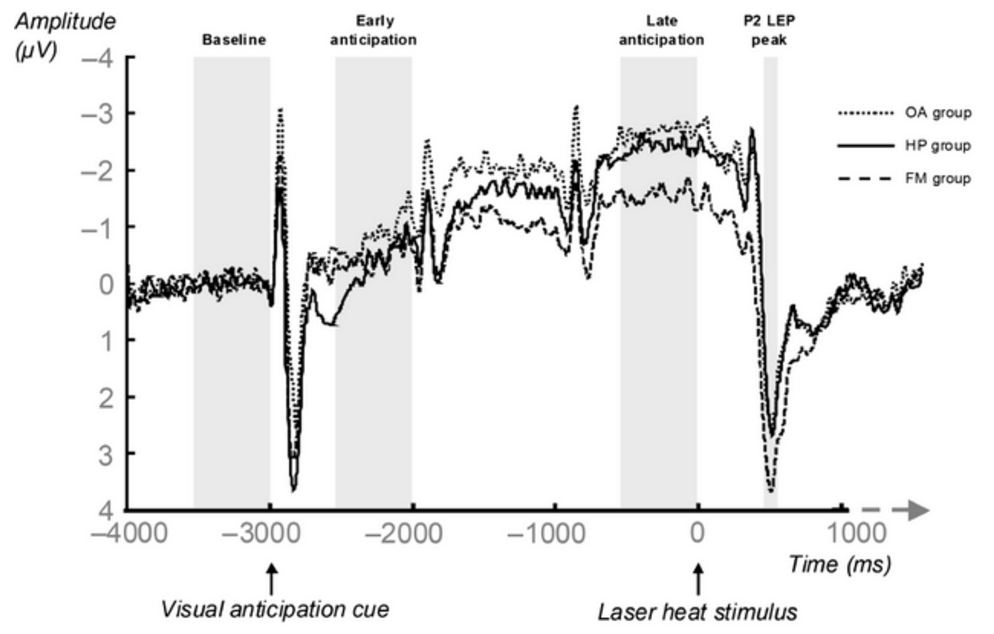
\includegraphics[width=0.7\textwidth]{figures/bProblemanalyse/EEG_ERP}
	\end{center}
	\caption{Figuren illustrerer de gennemsnitlige målinger for de tre forsøgsgrupper. Tidspunkter for måling af baseline, tidlig forventning, sen forventning og oplevelse af smerte er angivet på figuren. \citep{Brown2013}} 
	\label{fig:EEG_gns} 
\end{figure} 
Ud fra resultaterne var det muligt at undersøge i hvilke områder, der forekom særlig aktivitet ved hjælp af blandt andet billeddannende programmer. Resultaterne for studiet antyder, at de to patientgrupper responderer ens på forventningen om smerte, på trods af, at fibromyalgipatienternes respons var kraftigere. Disse resultater indikerer, at denne tendens kan være generelt gældende for patienter med kroniske smerter. \citep{Brown2013} Udgifterne til EEG-undersøgelse omfatter indkøb af udstyr samt løn til medarbejderne, der er med til at udføre undersøgelsen\citep{Green1985}.  
 % 1 = fMRI techniques and protocols
 % 2 = The dorsolateral prefrontal network is involved in pain perception in knee osteoarthritis patients
 % 3 = Brain activity for chronic knee osteoarthritis: dissociating evoked pain from spontaneous pain
 % 4 = Quantitative sensory testing
 % 5 = The evolution of primary hyperalgesia in orthopedic surgery: Quantitative sensory testing and clinical evaluation before and after total knee arthroplasty
 % 6 = Clinical electrophysiology
 % 7 = When the brain expects pain: common neural responses to pain anticipation are related to clinical pain and distress in fibromyalgia and osteoarthritis 
 %10 = Benefits, Shortcomings, and Costs of EEG Monitoring
\newpage \section{Problemafgrænsning}
Selvom operationerne bliver udført ‘perfekt’ så er 11 til 25\% af patienterne stadig utilfredse. Det tyder på at disse patienter er utilfredse pga. deres manglende resultater efter operationen, relateret til smerte og funktionsnedsættelse. Klinikerne er ansvarlig for belsutningstagen hvorvidt en patient er egnet til at modtage en TKA-operation. Klinikerne formår succesfuldt at udvælge 75 til 81\% af patienterne, på baggrund af deres erfaring, radiologiske fund, symptom vurdering, samt patientens egne udtalelser. Den resterende patientgruppe er utilfredse med resultatet, hvilket indikerer at udvælgelsesmetoden ikke er god nok, og at eventuelle bias kan have medvirket til dette resultat. Det kunne derfor, for klinikeren og patienten være fordelagtigt hvis den benyttede metode blev optimeret. Optimeringen kunne indebære afbenyttelse af en teknologisk metodik. Den teknologiske tilgang skulle medføre nogle faktiske resultater som skal supplere og bidrage til klinikerens beslutningstagen. Hvis en teknologisk metode skal kunne implementeres kræves det at denne muliggør identificering af patientgruppen, hvis risiko for kroniske komplikationer postoperativt, er størst. Den teknologiske tilgang bør ydermere være minimalt invasiv, omkostningseffektiv og let organisatorisk implementerbar. Disse kriterier opfyldes på bedste vis af QST, blandt de analyserede smertediagnosticeringsmetoder, hvormed det antydes at QST vil være den teknologiske tilgang som bedst vil kunne supplere klinikerens beslutningstagen. 

\subsection{Problemformulering}
\begin{center}
	\textit{Hvilke konsekvenser er der forbundet med en implementering af QST som supplement til klinikerens vurdering af patienten til indstilling til TKA, på de ortopædkirurgiske afdelinger i Region Nordjylland?}
\end{center}
\cleardoublepage
%\chapter{Syntese}\vspace{-.75cm}
%%\input{rapportAfsnit/../..}

\begingroup
\label{litteraturliste}
\raggedright
\bibliographystyle{unsrtnat}
\bibliography{kilder}
\endgroup
\begin{appendices}
%	\input{rapportAfsnit/qBilag/pilotforsoeg}
%	\input{rapportAfsnit/qBilag/MCU}
\end{appendices}

\end{document}
